\documentclass[12pt,a4paper]{article}
\usepackage{amsmath}
\usepackage{geometry}
\usepackage{graphicx}
\usepackage{tikz}
\usepackage{hyperref}

\geometry{margin=1in}

\title{The Circumscribed Circle of a Triangle}
\author{Tutoring Centre Ferndale\\

\includegraphics[width=4em]{ApS_logo.png}}
\date{}

\begin{document}

\maketitle

In geometry, the \textbf{circumscribed circle} of a triangle, also known as the \textbf{circumcircle}, is the unique circle that passes through all three vertices of the triangle. It is an important concept in triangle geometry and has various applications in trigonometry and coordinate geometry.

\section*{Definitions}

\subsection*{Circumscribed Circle}
The circumscribed circle of a triangle is the circle that contains all three vertices of the triangle. Every triangle, whether it is scalene, isosceles, or equilateral, has exactly one unique circumscribed circle.

\begin{center}
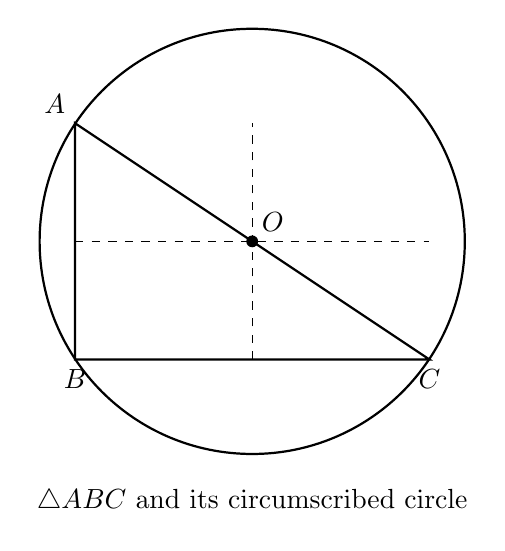
\begin{tikzpicture}[scale=1.5]
    \coordinate [label=above left:$A$] (A) at (0, 2);
    \coordinate [label=below:$B$] (B) at (0, 0);
    \coordinate [label=below:$C$] (C) at (3, 0);
    \coordinate [label=above right:$O$] (O) at (1.5, 1);
    \draw [thick] (O) circle [radius=1.8];
    \draw [thick] (A) -- (B) -- (C) -- cycle;
    \draw [dashed] (0,1) -- (3,1);
    \draw [dashed] (1.5, 0) -- (1.5, 2);
    \fill (O) circle [radius=0.05];
    \node at (1.5,-1.2) {\( \triangle ABC \) and its circumscribed circle};
\end{tikzpicture}
\end{center}

\newpage

\subsection*{Circumcenter}
The \textbf{circumcenter} is the center of the circumscribed circle. It is the point where the \textbf{perpendicular bisectors} of the sides of the triangle meet. The circumcenter has the following properties:
\begin{itemize}
    \item It is equidistant from all three vertices of the triangle.
    \item Its location depends on the type of triangle:
    \begin{itemize}
        \item For an \textbf{acute triangle}, the circumcenter lies inside the triangle.
        \item For a \textbf{right triangle}, the circumcenter lies on the hypotenuse.
        \item For an \textbf{obtuse triangle}, the circumcenter lies outside the triangle.
    \end{itemize}
\end{itemize}

\subsection*{Circumradius}
The radius of the circumscribed circle is called the \textbf{circumradius}, denoted by \( R \). It can be calculated using the formula:
\[
R = \frac{a \cdot b \cdot c}{4 \cdot \text{Area of the triangle}}
\]
where \( a \), \( b \), and \( c \) are the side lengths of the triangle.

\section*{Properties of the Circumscribed Circle}

\begin{enumerate}
    \item The circumcircle contains all three vertices of the triangle.
    \item The perpendicular bisectors of the sides intersect at the circumcenter, which is the center of the circle.
    \item The circumradius \( R \) is related to the sides and angles of the triangle through the \textbf{Law of Sines}:
\[
\frac{a}{\sin A} = \frac{b}{\sin B} = \frac{c}{\sin C} = 2R
\]
\end{enumerate}


\end{document}